\documentclass[]{article}
\usepackage{amsmath}
\usepackage{amsfonts}
\usepackage{amssymb}
\usepackage{hyperref}
\usepackage{gensymb}
\usepackage{graphicx}
\usepackage{svg}
\usepackage{bbding}
\usepackage{mathtools}
\usepackage{centernot} % not parallel, etc.
\usepackage{lmodern}
\usepackage{morewrites}
\usepackage{xcolor,sectsty} % colorful sections
\usepackage[left=10mm, top=10mm, right=10mm, bottom=20mm, nohead]{geometry}
%\usepackage{bigints}
\usepackage{dsfont} %mathbb 1
\usepackage{esint} % beatiful integrals
\usepackage{physics}


\DeclareFontFamily{OMX}{lmex}{}
\DeclareFontShape{OMX}{lmex}{m}{n}{<-> lmex10}{}


%colors of sections
\definecolor{secfont}{RGB}{46,116,181}
\definecolor{subfont}{RGB}{146,23,57}
\definecolor{parfont}{RGB}{19,127,43}
\definecolor{subparfont}{RGB}{7,11,100}

\subsectionfont{\color{subfont}}
\sectionfont{\color{secfont}}
\paragraphfont{\color{parfont}}
\subparagraphfont{\color{subparfont}}

%\usepackage{babel}[english]
%opening
\title{114036 - Statistical and Thermal Physics}
\author{Amit Keren}
% Wednesday 304, 16:00
% send notes
% Midterm - 5 lists, Final 10 lists
% Book Kittel Statermit

\parindent=0em
\begin{document}


\maketitle

\begin{abstract}

\end{abstract}

%\tableofcontents
\section{Introduction}
\paragraph{History}
\begin{itemize}
	\item First, thermodynamics was developed, before atoms were known to exist.
	\item Statistical physics.
	\item Quantum physics. 
\end{itemize}
In the course, the order is the opposite.
\subsection{}
Suppose we have two balls of diameter $d$. If both are on the bottom, total energy is 0. If one i son the other, total energy is $mgd$.

\begin{center}
	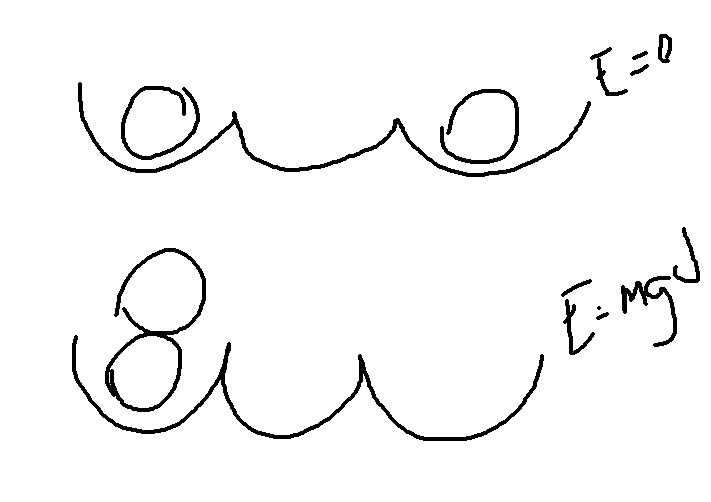
\includegraphics[width=0.5\linewidth]{./lect1/pic1.png}
	
	\begin{tabular}{c|c|c}
		Number of state & Degeneracy & Energy \\\hline
		0 & 3 & 0 \\
		1 & 3 & $mgd$ \\
		2 & 0 & $2mgd$ \\
	\end{tabular}
\end{center}
\paragraph{Paramagnetism}
Define magnetic moment as $\vec{m} = I \vec{a}$.
For magnetic filed energy is $U = -\vec{B} \cdot \vec{m} = - \vec{B} \dot \vec{\mu}$.

Suppose we a have a system of a big amount of current loops, each of which can have one of two directions - clockwise or counterclockwise. For example

\begin{center}
	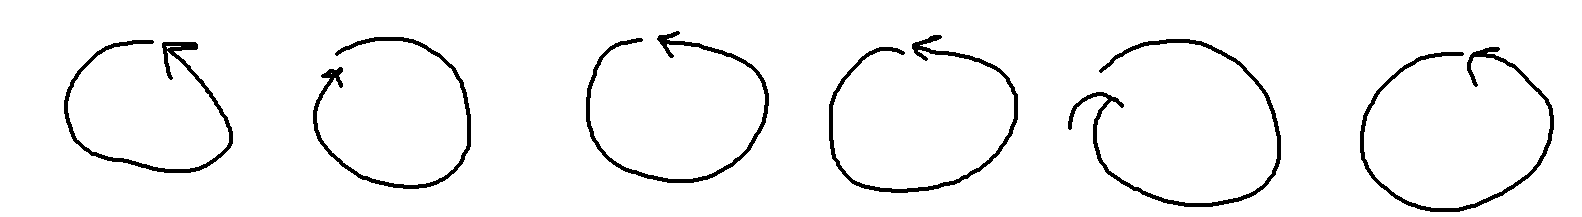
\includegraphics[width=0.5\linewidth]{./lect1/pic2.png}
\end{center}
To calculate total magnetic momentum we just sum all of the moments, which are either $\mu$ or $-\mu$. In upper example, $M = \sum_i \mu_i = 2\mu$.


The total number of possible states is $2^N$. The possible energy is $M = (N-2N_d)\mu$ where $N_d$ is number of down-facing loops of current. Number of different states with sam energy is $$\binom{N}{N_d} = \frac{N!}{N_d!N_u!}$$

Now, for even $N$, define 
$$2S = N_u -N_d$$
Then
$$\binom{N}{N_d} = \frac{N!}{(\left(\frac{1}{2} N - S\right)!(\left(\frac{1}{2} N + S\right)!}$$
and the energy
$$U = -2S\mu B \Rightarrow S = -\frac{U}{2\mu B}$$
The degeneracy of the state thus is
$$g(N,S) = \frac{N!}{\left(\frac{1}{2} N - \frac{U}{2\mu B}\right)!(\left(\frac{1}{2} N + \frac{U}{2\mu B}\right)!}$$ 
\paragraph{Particles on shelves (quantum oscillator)}
Suppose we have equally-distant shelves, and energy distance between two shelves is $\epsilon_0$:
\begin{center}
	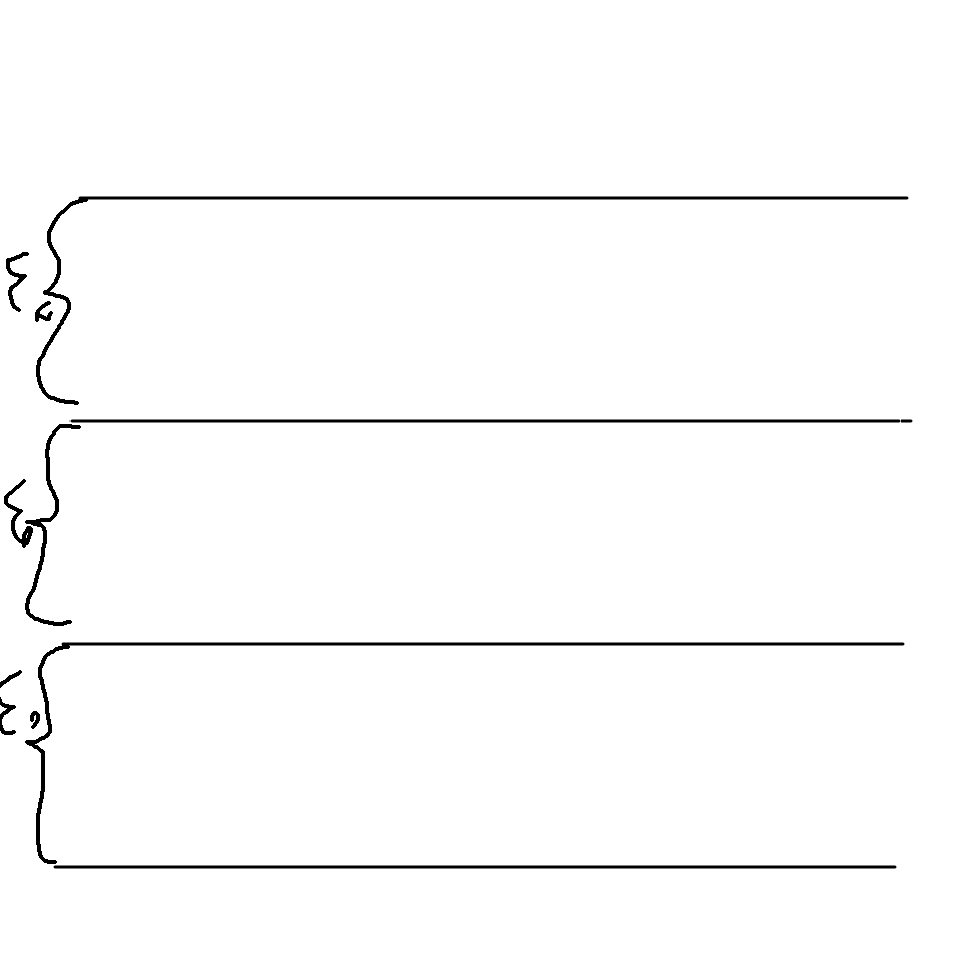
\includegraphics[width=0.5\linewidth]{./lect1/pic3.png}
\end{center}
Define $n=\frac{U}{\epsilon_0}$ which is amount of energy we have (it comes in quantas is degeneracy? What is degeneracy? It is combinations of$N$ out $n$ with returns:
$$g(N,u) = \frac{(n+N-1)!}{n!(N-1)!} = \frac{\left(N+\frac{U}{\epsilon_0} - 1\right)!}{\left(\frac{U}{\epsilon_0}\right)!(N-1)!}$$

\paragraph{Particles on shelves with quadratic distances (particles in box)}
Now suppose distances goes as square of number opf shelve ($\epsilon_0$, $4\epsilon_0$, ...). This problem doesn't have analytical solution. But we can find solution manually. For example, to find $g(6,18\epsilon_0)$. The only option is 2 boxes on first energy level $U=\epsilon_0$ and 4 on second energy level, thus 
$$g(6, 18\epsilon_0) = \binom{6}{2}=15$$  
\paragraph{1D box with particles}
Now we want to calculate kinetic energy:
$$E = \frac{p^2}{2m}$$
Since we can't do much with continuous values (there is infinite number of options), lets divide both momentum and position into discrete intervals of size $w$ and $l$ correspondingly. Now, the position is independent on energy, but there are only two options for momentum - $\pm \sqrt{2mE}$. Thus degeneracy is
$$g(1, E) = 2\frac{L}{l} $$
\paragraph{2D box}
We now divide position in momentum into intervals of length $l$ and $w$ in both directions. Position is still arbitrary, and momentum lies on a circle of radius $2mE$. However, its hard to calculate.

Lets define instead $S(1,E)$ - number of states with energy \textit{less} than $U$. For 1-dimensional case 
$$S(1,E)  = \frac{L}{l} \cdot 2 \cdot \frac{\sqrt{2mE}}{w} = \frac{1}{lw} \int_{-\frac{L}{2}}^{\frac{L}{2}} ds \int_{-\sqrt{2mE}}^{\sqrt{2mE}} ds$$
In 2D we get, for box of area $A$
$$S(1,E) = \frac{A}{l^2} \cdot \frac{2\pi m E}{w^2} =  \frac{1}{l^2w^2} \int_{-\frac{L}{2}}^{\frac{L}{2}}dx\int_{-\frac{L}{2}}^{\frac{L}{2}}dy \iint\limits_{|p| < \sqrt{2mE}} d^2p$$
$$S(1,E) = \frac{V}{l^3} \cdot\frac{4\pi (2 m E)^{\frac{3}{2}}}{3w^3}$$
We denote $h=lw$.
Now note that $G(n, U) = \pdv{S(n,U)}{U}$.

\paragraph{Two distinguishable particles in 1D}

While positions are independent, there is dependence between $p_1$ and $p_2$:
$$\frac{p_1^2}{2m}+\frac{p_2^2}{2m} + E$$
We can note that
$$S_{2D}(1,U) = S_{1D} (2, U)$$

\paragraph{$N$ particles in $D$ dimensions}
$$S_D(N,U) = \frac{1}{h^{DN}} \int\limits_{\va{x}_1 \in V} \dd[D]{x_1} \: \dots  \int\limits_{\va{x}_n \in V} \dd[D]{x_n}  \idotsint\limits_{\sum_{i=1}^n \va{p}_i^2 \leq 2mU} \dd[D]{p_1} \dots \dd[D]{p_n}$$

\subparagraph{Ball volume in dimension $d$}
Define gamma function. For $\alpha > 0$
$$\frac{1}{\alpha} = \int_0^\infty \dd{x} e^{-x\alpha}$$
Differentiating $n$ times by $\alpha$ (and dividing by $(-1)^n$:
$$\frac{N!}{\alpha^{N+1}} = \int_0^\infty \dd{x} x^N e^{-x\alpha}$$
By substituting $\alpha = 1$:
$$N! = \int_0^\infty \dd{x} x^N e^{-x}$$
Thus define 
$$\Gamma(N+1) = \int_0^\infty \dd{x} x^n e^{-x}$$

Define area of $d$-dimensional sphere of radius $R$ as
$$A_d = S_d \cdot R^{d-1}$$
Define also
$$I_d = \left(\int_{-\infty}^{\infty} \dd{x} e^{-x^2}\right)^d$$
On one hand $I_D = \pi^{\frac{d}{2}}$, on the other hand
$$I_d = \int_{-\infty}^{\infty} \dd{x_1}  e^{-x^2} \int_{-\infty}^{\infty} \dd{x_2}  e^{-x^2} \dots \int_{-\infty}^{\infty} \dd{x_n}  e^{-x^2} = \int_{-\infty}^{\infty} \dd{x_1}\dd{x_2}\dots \dd{x_n}   e^{-\sum_{i=1}^n x_i^2}$$
For $R=\sum_{i=1}^n x_i^2$:
$$I_D = \int_0^\infty \dd{R} S_d R^{d-1} e^{-R^2}$$
(Note that when we perform integral over angular dimensions we acquire exactly $S_d$ from Jacobean).

For $y=R^2$, $\dd{y}=2R\dd{R}$:
$$\int_0^\infty \frac{dy}{2\sqrt{y}} S_d y^{\frac{d-1}{2}} e^{-y} = \frac{S_d}{2} \int_{0}^{\infty} y^{\frac{d}{2} -1} e^{-y} dy = \frac{S_d}{2} \Gamma\left(\frac{d}{2}\right)$$
Thus
$$\frac{S_d}{2} \Gamma\left(\frac{d}{2}\right) = \pi^{\frac{d}{2}} $$
i.e.\
$$S_d = \frac{2\pi^{\frac{d}{2}}}{\Gamma\left(\frac{d}{2}\right)}$$

Now the volume of $d$-dimensional ball
$$V_d = \int_0^R \dd{r} \frac{2\pi^{\frac{d}{2}}}{\Gamma\left(\frac{d}{2}\right)} r^{d-1}= \frac{\pi^{\frac{d}{2}}}{\Gamma\left(\frac{d}{2}\right)} \frac{r^{d}}{\frac{d}{2}}= \frac{\pi^{\frac{d}{2}}r^{d}}{\Gamma\left(\frac{d}{2}+1\right)}$$

Back to our particles:

$$S_D(N,U) = \frac{1}{h^{DN}} \int\limits_{\va{x}_1 \in V} \dd[D]{x_1} \: \dots  \int\limits_{\va{x}_n \in V} \dd[D]{x_n}  \idotsint\limits_{\sum_{i=1}^n \va{p}_i^2 \leq 2mU} \dd[D]{p_1} \dots \dd[D]{p_n} = \frac{L^{DN} \pi^{\frac{DN}{2}} (2mU)^{\frac{DN}{2}}}{h^{DN} \Gamma\left(\frac{DN}{2}+1\right)} = \left(\frac{L}{h}\right)^{DN}\frac{  (2\pi mw)^{\frac{DN}{2}}}{\Gamma\left(\frac{DN}{2}+1\right)}$$

Thus in our world 
$$S_3(N,U) = \frac{V^{N} \pi^{\frac{3N}{2}} (2mU)^{\frac{3N}{2}}}{h^{3N} \Gamma\left(\frac{3N}{2}+1\right)}$$
And
$$G_3(N,U) = \pdv{S_3(N,U)}{U} = \frac{V^{N} \pi^{\frac{3N}{2}} (2mU)^{\frac{3N}{2}-1} \cdot \frac{3}{2}N \cdot 2m}{h^{3N} \Gamma\left(\frac{3N}{2}+1\right)} = \frac{3V^{N} \pi^{\frac{3N}{2}} (2mU)^{\frac{3N}{2}-1}mN}{h^{3N} \Gamma\left(\frac{3N}{2}+1\right)}$$

\paragraph{Integral approximation with steepest descent}
Suppose we want calculate 
$$I = \int \dd{x} e^{N \phi(x)}$$
for some big $N$ and $x_{max}$ is maximum of $\phi$:
$$I \approxeq \int \dd{x} \exp\left[N \left(\phi(x_{max}) - \frac{1}{2} \left| \phi''(x_{max}) \right| (x-x_{max})^2 + \frac{1}{3!} \phi'''(x_{max} ) (x-x_{max})^3 \right)\right]$$
Then, substituting $y=\sqrt{N}(x-x_{max})$
$$I = e^{N\phi(x_{max})} \int \frac{\dd{y}}{\sqrt{N}} e^{-\frac{1}{2} |\phi''(x_{max})| y^2 + \frac{1}{3!}\phi''' \left(x_{max}\right)\frac{y^3}{\sqrt{N}}}$$
Since $N$ is big, $\frac{1}{3!}\phi''' \left(x_{max}\right)\frac{y^3}{\sqrt{N}}$ is negligible (and higher orders too):
$$I =  e^{N\phi(x_{max})} \sqrt{\frac{2\pi}{N |\phi''(x_{max})|}}$$

\subparagraph{Example}
Lets approximate $n!$:
$$\Gamma(n+1) = \int_0^\infty \dd{x} x^N e^{-x} = \int_0^\infty \dd{x} e^{N \left( \ln x - \frac{x}{N}\right)}$$
Thus $\phi(x) = \ln x - \frac{x}{N}$, and
$$\phi'(x)  = \frac{1}{x} - \frac{1}{N}$$
i.e., $x_{max} = N$. And
$$\left|\phi''(x) \right| = \frac{1}{x^2} $$
$$\Gamma(n+1) = \int_0^\infty \dd{x} x^N e^{-x} = \int_0^\infty \dd{x} e^{N \left( \ln x - \frac{x}{N}\right)} \approxeq e^{N\left( \ln N - 1\right)} \sqrt{\frac{2\pi}{N \frac{1}{N^2}}} = N^N e^{-N} \sqrt{2 \pi N}$$
which is Stirling approximation. We usually want to take logarithm:
$$\ln (N!) \approxeq N\ln N - N + \frac{1}{2} \ln (2\pi N)$$
\paragraph{Example}
Back to example with up and down particles:
$$g(N,S) = \frac{N!}{N_{\uparrow}!N_\downarrow!}$$
where $2S = N_\uparrow - N_\downarrow$ and $N= N_\uparrow + N_\downarrow$
$$\ln g = \ln N! - \ln N_\uparrow ! - \ln N_\downarrow!$$
$$\ln N! = \frac{1}{2} \ln 2\pi + (N+1) \ln N - \frac{1}{2} \ln N - N$$
Substituting
$$\ln N! = \frac{1}{2}ln \frac{2\pi}{N} + \qty(N_\uparrow + \frac{1}{2} + N_\downarrow + \frac{1}{2}) \ln N - (N_\uparrow + N_\downarrow)$$
in addition
$$\ln N_\uparrow! = \frac{1}{2} \ln 2\pi + \qty(N_\uparrow + \frac{1}{2}) \ln N_\uparrow - N_\uparrow$$
$$\ln N_\downarrow! = \frac{1}{2} \ln 2\pi + \qty(N_\downarrow + \frac{1}{2}) \ln N_\downarrow - N_\downarrow$$
so
$$\ln g = \frac{1}{2}ln \frac{1}{2\pi N}  - \qty(N_\uparrow - \frac{1}{2}) \ln \frac{N_\uparrow}{N}   - \qty(N_\downarrow + \frac{1}{2}) \ln \frac{N_\downarrow}{N} $$
Now since
$$\ln \frac{N_\uparrow}{N} = \ln(\frac{1}{2} + \frac{2S}{2N}) = \ln\frac{1}{2}\qty(1 + \frac{2S}{N}) = \ln \frac{1}{2} + \ln(1+\frac{2S}{N})$$
If $S \ll N$
$$\ln \frac{N_\uparrow}{N}  = -\ln 2 + \frac{2S}{N} - \frac{2S^2}{N^2}$$
similarly
$$\ln \frac{N_\downarrow}{N}  = -\ln 2 - \frac{2S}{N} + \frac{2S^2}{N^2}$$
Thus
$$\ln g = \frac{1}{2}ln \frac{1}{2\pi N}  - \qty(\frac{1}{2}N + S - \frac{1}{2}) \qty(-\ln 2 + \frac{2S}{N} - \frac{2S^2}{N^2})  - \qty(\frac{1}{2}N - S + \frac{1}{2}) \qty(-\ln 2 - \frac{2S}{N} +  \frac{2S^2}{N^2}) $$
i.e.,
$$\ln g = \frac{1}{2}ln \frac{2}{\pi N}  + N \ln 2 -\frac{2S}{N} + \order{\frac{S^3}{N^2}}$$
$$g(N,S) = \qty(\frac{2}{\pi N})^{\frac{1}{2}} 2^N e^{-\frac{2S^2}{N}}$$
And if use energy,
$$g(N, U) = \qty(\frac{2}{\pi N})^{\frac{1}{2}} 2^N e^{-\frac{2U^2}{(\mu B)^2N}}$$

Now since number of configurations is $2N$, 
$$\rho(S) = \qty(\frac{2}{\pi N})^{\frac{1}{2}} e^{-\frac{2S^2}{N}} $$
Which is normal distribution with mean $0$ and standard deviation $\frac{\sqrt{N}}{2}$.

Lets check the standard deviation of actual $S$:
$$\langle (2S)^2 \rangle = \left\langle \qty(\sum_i N_i) \right\rangle = \left\langle \sum_{i,j} N_iN_j \right\rangle = \left\langle \sum_i N_i^2 \underbrace{\sum_{i\neq j} N_iN_j}_{0 \: \text{from independence}} \right\rangle  =\left\langle \sum_i N_i^2\right\rangle = N$$
Thus variance of $2S$ is $N$ and variance of $S$ is $\frac{N}{4}$. (This is immediate from CLT).
\end{document}
